 Halo semua dan selamat datang di kursus Neural Convolutional, dengan pembelajaran python bagian 9. Neural Convolutional adalah salah satu kursus yang menarik dan membuktikan bahwa siswa yang mengikuti kursus ini akan lebih cepat dan mudah mengerti. Saya akan memberikan pembelajaran tentang pendalaman materi yang dapat membantu anda dalam pembelajaran  dengan banyaknya materi- materi.
Jadi, izinkan saya menjelaskan dengan secara  singkat tentang kursus ini	:

 Dalam kursus ini kita akan mempelajari bagaimana cara mengatur antara arsitektur CNN dasar yang sudah anda kenal dan menikmati arsitektur novel modern seperti Viji Reznick dan Inception yang mungkin akan anda beri sesuai nama film. Kami akan menggunakan ini pada gambar sel sel dan membuat sistem yang lebih baik.
 Salah satu tema utama dari kursus ini juga beralih dari CNN ke sistem yang melibatkan CNN. CNN juga membuat satu gambar klasifikasi hal dasar dalam kursus ini, anda akan melihat bagaimana kita dapat mengubah CNN menjadi sistem deteksi objek yang tidak hanya mengklasifikasikan gambar tetapi juga dapat menemukan setiap objek dalam gambar dan prediksi labelnya.



\section{Jaringan saraf convolutional canggih}
Tujuan Pembelajaran
\begin{enumerate}

\item  kita telah melihat bahwa 3-5 layer netscan membutuhkan waktu yang sangat lama untuk dilatih
(tapi sekarang kita akan melihat 50 layer nets)
\item penelitian hari ini (dalam pembelajaran mesin) berkomitmen untuk keterbukaan, dan dengan membagikan penelitian mereka, mudah bagi Anda untuk melakukan hal-hal canggih di rumah
(Tidak ada bidang lain yang bisa mencapai ini: biologi, kedokteran, fisika, ...dan lain sebagainya)
\item kita dapat menggunakan bobot pra-terlatih menggunakan transfer belajar secara signifikan mengurangi waktu pelatihan karena kita sekarang hanya perlu melakukan fine-tuning
\end{enumerate}

\section{cara untuk melakukan kursus ini dengan baik}
Saya telah menemukan solusi ini setelah mengamati siswa/i selama bertahun-tahun,
pada umumnya, mereka yang mengikuti solusi ini telah mendapatkan kesuksesan, mereka yang memiliki masalah disebabkan karena tidak mengikuti solusi ini.

Hal-hal atau solusi yang diperlukan antara lain :
\begin{enumerate}
\item memanfaatkan dengan adanya Question and Answer  
\item memerlukan waktu respon yang cepat
\item mempunyai motifasi yang tinggi
\item menggunakan sotfware yang kita mengerti dan kita pahami 
\end {enumerate}


\section{Convolutional Neural Network}
Ulasan tentang CNN
\begin{enumerate}

\item Memahami penulisan jaringan saraf feedforward menggunakan beberapa pustaka
\item Mengetahui secara umum bagaimana jaringan saraf bekerja, bagaimana melatihnya pada data, seperti apa data itu (formatnya), bagaimana membuat prediksi baru tentang data tersebut.
\item Mengetahui tentang convolution
\end{enumerate}

Convolution
\begin{enumerate}
\item Filter(3X3) adalah tensor berat yang dipelajari dengan backpropagation.
\item Kesalahan : merancang filter untuk menjadi pendeteksi tepi dll.
\item Tidak dapat diskalakan: CNN berisi seribuan filter saraf sehingga tidak mungkin anda dapat memperbaiki dengan cara yang dapat dilakukan sesuai kebutuhan anda
\end{enumerate}

\begin{figure}[!htp]
	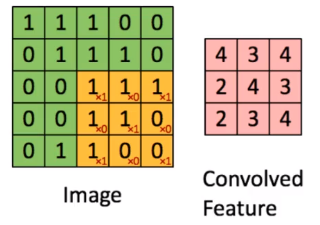
\includegraphics[width=0.75\textwidth]{figures/convolusi.PNG}
	\caption{Ilustasi gambar pada setiap pergeseran filter}
	\label{labelgambar}
\end{figure}
	Convolutional Neural Network (CNN) adalah salah satu jenis neural network yang biasa digunakan pada data image. CNN bisa digunakan untuk mendeteksi dan mengenali object pada sebuah image.
Secara garis besar CNN tidak jauh beda dengan neural network biasanya. CNN terdiri dari neuron yang memiliki weight, bias dan activation function.
Filter pada dasarnya meluncur diatas setiap posisi yang mungkin pada gambar dan pada setiap bagian yang tumpang tindih mendapatkan elemen berlipat ganda untuk pengadaan dan penambahan konvolusi ini merupakan konsep matrix seperti teknik pengukuran jarak ataupun mengukur korelasi sebuah matrix 
Jika filter sangat berkolerasi dengan potongan gambar maka akan menghasilkan jumlah yang sangat besar dan jika filter sangat berbeda dengan potongan gambar maka akan menghasilkan jumlah yang sangat kecil dalam aktualitas yang disebut konvolusi atau disebut sebagai korelasi silang karena konvolusi merupakan sebuah konsep 


\section{cara untuk mendapatkan kode dan data}
Langkahnya sebagai berikut
\begin{figure}[!htp]
	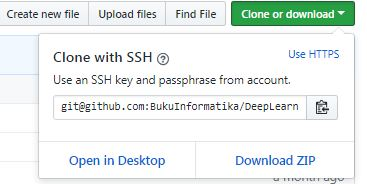
\includegraphics[width=0.75\textwidth]{figures/ssh.JPG}
	\caption{contoh pengambilan kode ssh}
	\label{labelgambar}
\end{figure}

\begin{enumerate}
\item mengambil kode ssh yang ada pada github dan pastikan yang dicopy adalah ssh bukan https
\item jangan lupa melakukan fork terlebih dahulu
\item kemudian disarankan untuk tidak memalsukan repo karena dapat mempersulit 
\end{enumerate}

Dalam hal data, data akan kita temui pada saat kita dalam kuliah dan kursus, beberapa siswa telah meminta saya untuk memberikan 
tentang tutorial latihan coding dalam kursus ini jadi tidak ada alasan lagi untuk tidak dapat mengoding

\begin{enumerate}
\item Jaringan saraf konvolutional canggih dalam kuliah ini saya akan membahas bagaimana untuk mendapatkan kode untuk kursus ini. Jadi seperti biasa kode dalam kursus ini dapat di unduh dari halaman saya. Untuk mendapatkan kunci tersebut, cobalah untuk mencoba dan menempelkan dari halaman web itu sendiri. Cukup gunakan perintah clone lalu buat semua folder yang relevan untuk kursus ini juga kelas CNN.
\item Tidak memalsukan report karena hal ini mempersulit untuk mendapatkan persetujuan dan saya membuat report yang cukup banyak dan terus menerus sehingga membuat anda tidak terjebak dengan versi lama. Selanjutnya jika anda sudah mengambil salah satu kelas saya dan anda sudah memiliki report ini cukup klik tarik dan anda secara otomatis memiliki kode untuk data dalam kursus ini.
\item Umumnya akan melihat data set yang berbeda, dimana untuk mendapatkan data didua tempat, baik dalam kuliah dan dalam kode. Jadi dalam kursus ini anda tidak perlu mengetik kode berulang kali hanya untuk melihat data set yang berbeda.
\end{enumerate}

\section{Data Fashion MNIST}
Data Fashion MNIST (Modified National Institute of Standards and Technology) adalah basis data yang berbentuk tulisan angka yang biasa digunakan untuk melatih pola pikir kita dalam algoritma.

Hal hal yang perlu kita lakukan untuk kursus Data Fashion MNIST :
\begin{enumerate}
\item Download terlebih dahulu kaggle pada google
\item Sebelum mendownload pastikan kamu telah memiliki akun kaggle 
\item Sediakan tempat penyimpanan file yang besar
\end{enumerate}

Kali ini kita akan melakukan contoh klasifikasi terhadap data Fashion MNIST. Fashion MNIST ini adalah dataset yang terdiri dari 10 kategori fashion sebagai berikut :
\begin{figure}[!htp]
	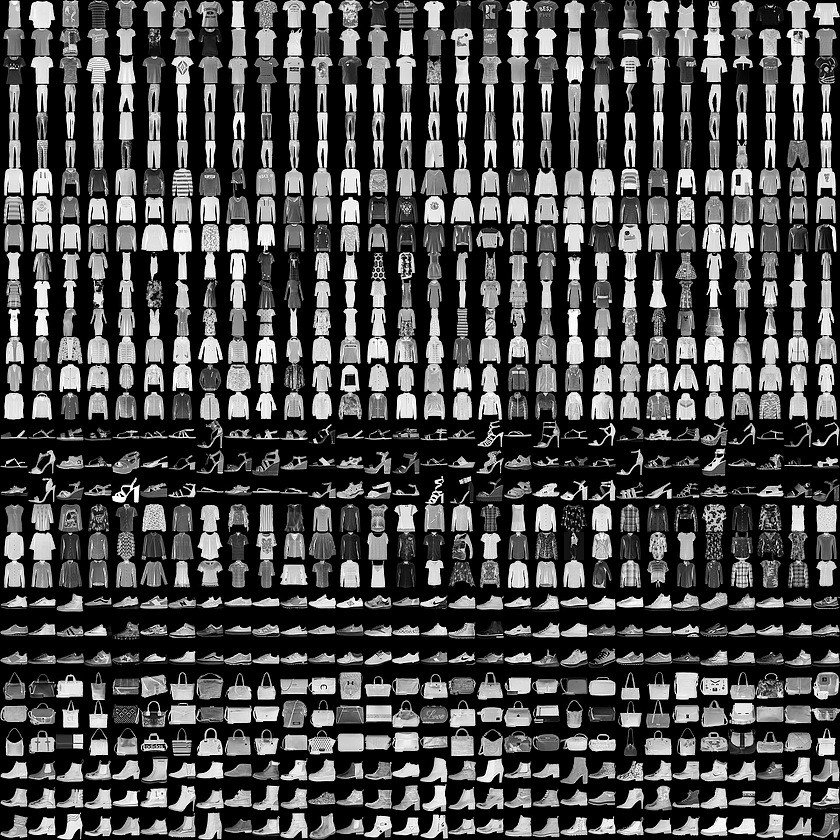
\includegraphics[width=0.75\textwidth]{figures/MNIST.PNG}
	\caption{contoh klarifikasi data Fashion MNIST}
	\label{labelgambar}
\end{figure}

\textbf{Hasil Klarifikasi}
\begin{enumerate}
\item T-Shirt/Tops = 0
\item Trouser = 1
\item Pullover = 2
\item Dress = 3
\item Coat = 4
\item Sandal = 5
\item Shirt = 6
\item Sneaker = 7
\item Bag = 8
\item Ankle Boot = 9
\end{enumerate}

Tiap kategori terdiri dari 6.000 images untuk training dan 1.000 images untuk testing. Jadi total untuk training data ada 60.000 images dan 10.000 untuk testing data.
 

\subsection{Dependency}
Dependency yang dibutuhkan pada contoh autoencoder kali ini hampir sama dengan contoh pada part-part sebelumnya. Hanya saja kali ini kita akan load MNIST data dari package yang sudah disediakan oleh Keras. Kita juga mau coba optimizers baru yaitu ADAM.

ADAM adalah variant dari algoritma gradient descent.
\begin{figure}[!htp]
	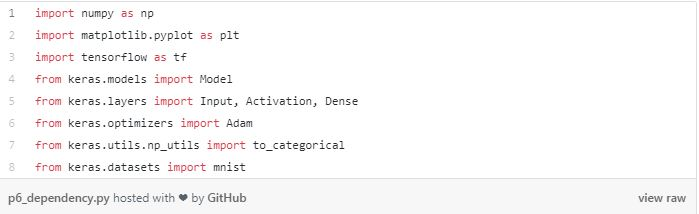
\includegraphics[width=0.75\textwidth]{figures/Dependency.JPG}
	\caption{contoh dependency}
	\label{labelgambar}
\end{figure}

\subsection{Data Preparation}
Data dari MNIST ini adalah grayscale image dengan range dari 0 hingga 255. Range data seperti ini “terlalu besar” untuk model kita, apalagi dengan learning rate yang cukup kecil, sehingga kita perlu melakukan scaling dengan membaginya dengan 255. Sehingga kita dapatkan range data baru antara 0 dan 1.


\section{Pengulasan tentang kode CNN}
Halo kembali lagi di materi jaringan Saraf Convolutional canggih, dalam kesempatan ini kita akan melihat bagaimana sebuah kode dapat digunakan untuk menerapkan CNN dan karies dengan menggunakan metode data amneris. Apa yang akan dipelajari adalah betapa mudahnya kode tersebut dapat membaca dokumentasi Cairnes selama beberapa menit. Jadi strategi dalam membuat data jaringan saraf pada dasarnya hanya mendeklarasikan daftar surat yang ingin dipelajari dengan jaringan yang hanya satu baris dan kemudian plot biaya dan metrik lainya, namun ini semua terlihat mudah karena hanya sebuah penjelasan. Sebelum memulai pembelajaraan ini, kita dapat melihat fashion yang tinggi di repo, seperti yang kita lihat diatas ada beberapa impor seperti jenis model yang kita inginkan secara berurutan dan semua jenis model yang diperlukan. Sebelumnya kami telah mempelajari semua jenis yang ada dimasa lalu sehingga kami dapat menemukan ide dan menggunakan untuk jenis model yang digunakan sekarang. Kami memiliki indikator untuk menentukan target yang berupa daftar indeks sehingga menjadi satu kesatuan yang berfungsi untuk mengategorikan data tersebut. jika pada dasarnya anda bisa menyalin kode apapun dari pembelajaraan sebelumnya yang dimuat dalam data yang sama yang akan dilakukan Karin. Untuk melakukan validasi split kereta. Tetapi disini saya mengacak-acak data untuk berjaga-jaga. Ingatlah bahwa kami ingin data berada dalam bentuk dan ketinggian dengan warna. Jadi kami membentuk ulang menjadi minus satu pada 28 satu. Karena gambar berukuran 28 x 28 dan skala abu-abu, kami juga ingin piksel gambar kami dinormalisasi sehingga kami membagi semuanya dengan 255 dan seperti halnya amnesti asli untuk mengatur label pada kolom pertama. Jadi X adalah segalanya mulai dari kolom 1 dan seterusnya. Dan mengapa semuanya ada di kolom 0. Selanjutnya kita mendapatkan K yang merupakan jumlah kelas dan pada baris berikutnya kita mengubah y menjadi matriks indikator sehingga kita dapat menggunakannya dalam cara yang sama dibagian kode selanjutnya.

\section{VGG-16}
\begin{figure}[!htp]
	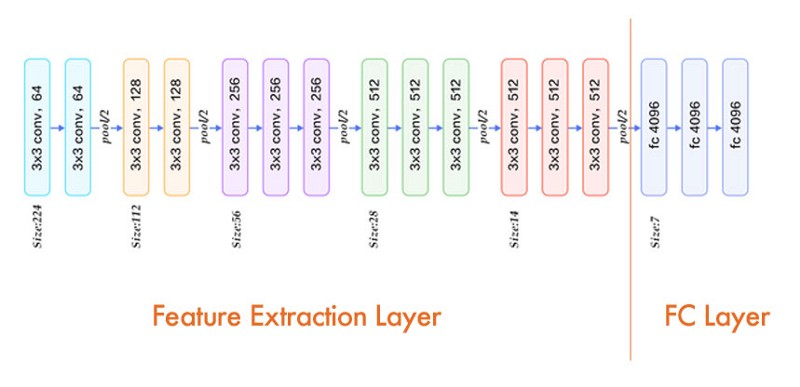
\includegraphics[width=0.75\textwidth]{figures/vgg.jpeg}
	\caption{gambar VGG-16}
	\label{labelgambar1}
\end{figure}

Gambar diatas adalah arsitektur dari VGG16 (16 Layer). Yang akan kita gunakan adalah Feature Extraction Layer saja, tentu saja dengan weights yang dapat kita download. Weights nya berupa file .h5 seperti yang sudah kita gunakan sebelumnya.

FC layer pada VGG16 terdiri dari 4096–4096–4096 neuron pada hidden layer dan 1000 neuron pada output layer karena ImageNet mempunyai 1000 classs. Sedangkan dataset kita hanya mempunyai 2 class (Male/Female), sehingga kita harus membuat FC layer versi kita sendiri.

Kita akan menggunakan FC Layer yaitu 32 neuron pada hidden layer dan 1 neuron pada output dengan sigmoid activation
( pada gambar \ref{labelgambar1} ).

\textbf{VGG-16 Dependiencies and variable} 

namun pada hal ini kita membutuhkan package applications untuk dapat menggunakan VGG16.

gambar dibawah adalah salah satu contoh source code pada package applications dari VGG-16 Dependiencies and variable ( pada gambar \ref{labelgambar2} ).
\begin{figure}[!htp]
	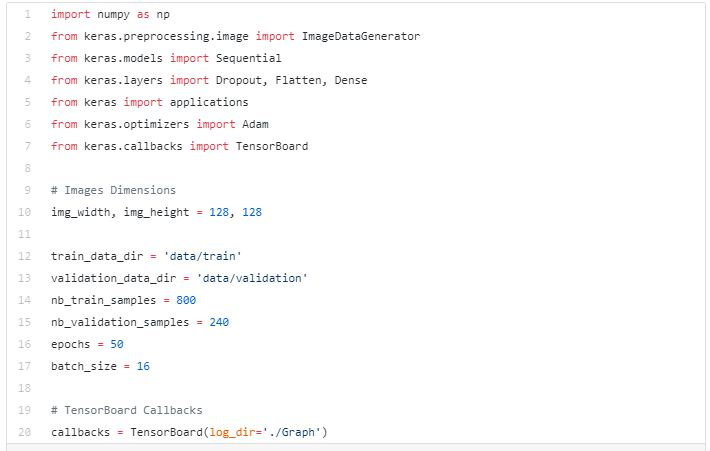
\includegraphics[width=0.75\textwidth]{figures/vgg1.jpeg}
	\caption{gambar VGG-16 Dependiencies and variable}
	\label{labelgambar2}
\end{figure}

\textbf{VGG-16 Model and Data Augmentation}

gambar dibawah adalah salah satu contoh source code pada package applications dari VGG-16 Model and Data Augmentation
( pada gambar \ref{labelgambar3} ).
\begin{figure}[!htp]
	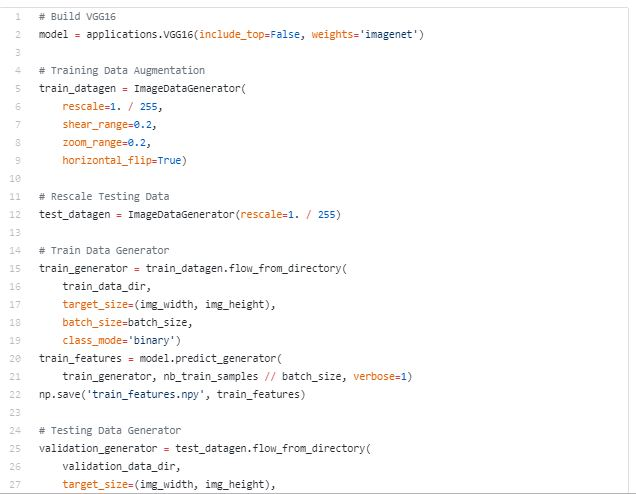
\includegraphics[width=0.75\textwidth]{figures/vgg2.JPG}
	\caption{gambar VGG-16 Model and Data Augmentation}
	\label{labelgambar3}
\end{figure}

Dengan menggunakan package applications kita bisa langsung menggunakan VGG-16 tanpa harus menyusunnya layer demi layer dan mendownload weights nya.

Argument include top sama dengan False diatas menandakan jika kita tidak menggunakan FC Layer dari VGG-16. Sehingga jika kita melakukan “predict” untuk model ini maka yang akan terjadi adalah dataset akan mengalir pada feature extraction layer dari VGG-16. 

Hasilnya adalah feature map yang bisa kita simpan pada file train features.npy dan val features.npy yang nantinya bisa kita flatten dan kita gunakan untuk melakukan training pada FC Layer versi kita sendiri.

\section{Convolutional Neural Network}
Convolutional Neural Network (CNN) adalah salah satu jenis neural network yang biasa digunakan pada data image. CNN bisa digunakan untuk mendeteksi dan mengenali object pada sebuah image.

Secara garis besar CNN tidak jauh beda dengan neural network biasanya. CNN terdiri dari neuron yang memiliki weight, biasa dan activation function seperti yang sudah kita pelajari pada part sebelumnya. Lalu apa yang membedakan? Arsitektur dari CNN dibagi menjadi 2 bagian besar, Feature Extraction Layer dan Fully-Connected Layer (MLP) 

\section{Feature Extraction Layer}
Saya gunakan istilah ini karena proses yang terjadi pada bagian ini adalah melakukan “encoding” dari sebuah image menjadi features yang berupa angka-angka yang merepresentasikan image tersebut (Feature Extraction).

Feature extraction layer terdiri dari dua bagian. Convolutional Layer dan Pooling Layer. Namun kadang ada beberapa riset/paper yang tidak menggunakan pooling(pada gambar \ref{labelgambar1} ).
\begin{figure}[!htp]
	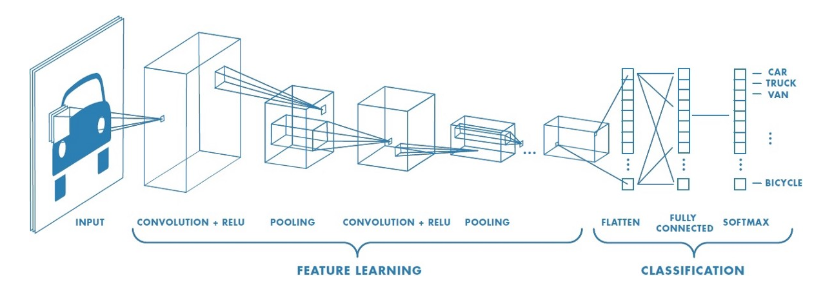
\includegraphics[width=0.75\textwidth]{figures/FeatureExtractionLayer.PNG}
	\caption{Contoh FEL}
	\label{labelgambar1}
\end{figure}

\section{Convolutional Layer}
 Gambar \ref{labelgambar2} adalah RGB (Red, Green, Blue) image berukuran 32x32 pixels yang sebenarnya adalah multidimensional array dengan ukuran 32x32x3 (3 adalah jumlah channel).
Convolutional layer terdiri dari neuron yang tersusun sedemikian rupa sehingga membentuk sebuah filter dengan panjang dan tinggi (pixels). Sebagai contoh, layer pertama pada feature extraction layer biasanya adalah conv. layer dengan ukuran 5x5x3. Panjang 5 pixels, tinggi 5 pixels dan tebal/jumlah 3 buah sesuai dengan channel dari image tersebut.
Ketiga filter ini akan digeser keseluruh bagian dari gambar. Setiap pergeseran akan dilakukan operasi “dot” antara input dan nilai dari filter tersebut sehingga menghasilkan sebuah output atau biasa disebut sebagai activation map atau feature map

 
\begin{figure}[!htp]
	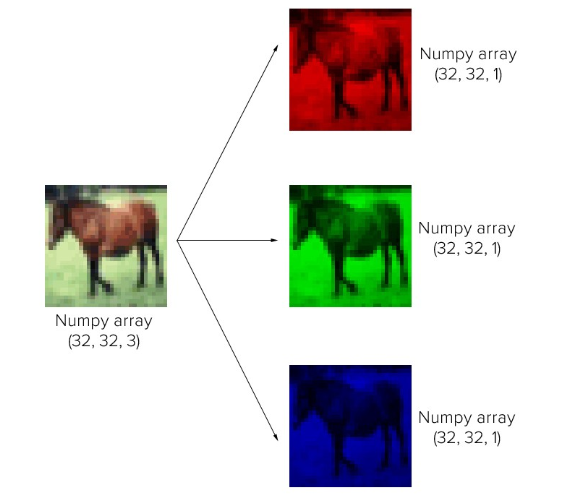
\includegraphics[width=0.75\textwidth]{figures/ConvolutionalLayer.PNG}
	\caption{Contoh CL}
	\label{labelgambar2}
\end{figure}

\section{Transfer Learning}
Transfer learning adalah suatu teknik atau metode yang memanfaatkan model yang sudah dilatih terhadap suatu dataset untuk menyelesaikan permasalahan lain yang serupa dengan cara menggunakannya sebagai starting point, memodifikasi dan mengupdate parameternya sehingga sesuai dengan dataset yang baru.

Kita akan gunakan model VGG-16 yang sudah dilatih pada data ImageNet dengan cara membuat arsitektur yang identik dengan VGG-16 tetapi tanpa fully-connected layer dan mendownload weights nya. Dengan menyediakan beberapa model ImageNet yang populer untuk bisa kita gunakan.

Seluruh weight VGG-16 telah dilatih menggunakan dataset ImageNet dan sudah dapat mengenali warna, tekstur, dll. Sehingga kita bisa manfaatkan ini untuk meng-extract feature dari semua foto pada dataset kita.